\documentclass [a4paper] {article}
\usepackage[hidelinks]{hyperref}
\usepackage[spanish,activeacute]{babel}
\usepackage[utf8]{inputenc}
\usepackage{amsmath}
\usepackage{graphicx}

\graphicspath{ {./imagenes/} }

\title{\textbf{Fundamentos de la Ciencia de Datos Práctica 1}}
\author{
	Fernández Díaz, Daniel.\\
	Cano Díaz, Francisco.\\
	Fernández Hernández, Alberto.\\
}

\date{15 de octubre del 2019}
\usepackage{Sweave}
\begin{document}
\maketitle

\section{Apartado 1}

Análisis estadístico de descripción de Datos en R. Para realizar este análisis utilizaremos dos ficheros de datos:
\begin{enumerate}
	\item \textbf{Fichero \textit{.txt}} con los datos de los satélites menores de Urano: nombre del satélite y su radio en km.
	\item \textbf{Fichero \textit{.sav}} (SPSS) formado por datos de automóviles, tales como su consumo en mpg (millas por galón), cilindrada, aceleración, año de fabricación, modelo etc.
\end{enumerate}

\subsection{Fichero \textit{.txt}}
Para comenzar a leer ficheros \textit{.txt} deberemos seguir una serie de reglas para generar el formato correcto:
\begin{itemize}
	\item Debe haber una tabulación entre dato y dato.
	\item Debe haber una primera columna que enumere las filas excepto la primera fila que tendrá un espacio en blanco. Además, en la primera fila irá el nombre de las variables.
	\item Hay que introducir un \textit{enter} al final de la última fila.
	\item Los decimales se introducen con punto.
	\item En las variables tipo caracter no se puede dejar un espacio entre caracteres.
\end{itemize}

\newpage

\begin{figure}
Siguiendo estas reglas generaremos un fichero con los datos de los satélites menores de Urano:

\centering
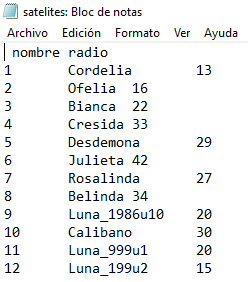
\includegraphics[width=3cm]{figura1}
\caption{Fichero \textit{.txt}.}
\end{figure}

Una vez creado el fichero nos disponemos a leer los datos que contiene. Para ello utilizaremos el comando \textbf{\textit{read.table}}:
\begin{Schunk}
\begin{Sinput}
> satelites <- read.table("satelites.txt")
> satelites
\end{Sinput}
\begin{Soutput}
         nombre radio
1      Cordelia    13
2        Ofelia    16
3        Bianca    22
4       Cresida    33
5     Desdemona    29
6       Julieta    42
7     Rosalinda    27
8       Belinda    34
9  Luna_1986u10    20
10     Calibano    30
11   Luna_999u1    20
12   Luna_199u2    15
\end{Soutput}
\end{Schunk}

Para llevar a cabo el análisis de los datos anteriores calcularemos las siguientes magnitudes:
\subsubsection{Frecuencia Absoluta y Acumulada}
Para calcular la frecuencia absoluta utilizaremos el comando \textbf{\textit{table}}:
\begin{Schunk}
\begin{Sinput}
> frecabsradio <- table(satelites$radio)
> frecabsradio
\end{Sinput}
\begin{Soutput}
13 15 16 20 22 27 29 30 33 34 42 
 1  1  1  2  1  1  1  1  1  1  1 
\end{Soutput}
\end{Schunk}
\newpage
Por otro lado, para calcular la frecuencia absoluta acumulada utilizaremos la frecuencia absoluta anterior y, con el comando \textbf{\textit{cumsum}}, realizaremos la suma acumulativa de las frecuencias absolutas:
\begin{Schunk}
\begin{Sinput}
> frecabsacmradio <- cumsum(frecabsradio)
> frecabsacmradio
\end{Sinput}
\begin{Soutput}
13 15 16 20 22 27 29 30 33 34 42 
 1  2  3  5  6  7  8  9 10 11 12 
\end{Soutput}
\end{Schunk}

\subsubsection{Frecuencia Relativa y Acumulada}
Para calcular la frecuencia relativa crearemos la siguiente función a través del comando \textbf{\textit{function}}. Esta función dividirá la frecuencia absoluta de cada dato entre el número total de datos:
\begin{Schunk}
\begin{Sinput}
> frecrel <- function(x) {table(x)/length(x)}
\end{Sinput}
\end{Schunk}

Una vez creada la función la guardamos en un fichero \textit{.R} a través del comando \textbf{\textit{dump}}, lo que nos permitirá cargarla en cualquier script que hagamos:
\begin{Schunk}
\begin{Sinput}
> dump("frecrel",file = "frecrel.R")
\end{Sinput}
\end{Schunk}

Para cargar scripts en \textit{.R} y poder utilizar sus funciones utilizaremos el comando \textbf{\textit{source}}:
\begin{Schunk}
\begin{Sinput}
> source("frecrel.R")
\end{Sinput}
\end{Schunk}

Una vez cargado calcularemos la frecuencia relativa:
\begin{Schunk}
\begin{Sinput}
> frecrelradio <- frecrel(satelites$radio)
> #Lo convertimos a dataframe para mostrarlo por pantalla de una forma más limpia
> df = data.frame(frecrelradio)
> print(df, row.names = FALSE)
\end{Sinput}
\begin{Soutput}
  x       Freq
 13 0.08333333
 15 0.08333333
 16 0.08333333
 20 0.16666667
 22 0.08333333
 27 0.08333333
 29 0.08333333
 30 0.08333333
 33 0.08333333
 34 0.08333333
 42 0.08333333
\end{Soutput}
\end{Schunk}
\newpage
Por otro lado, para calcular la frecuencia relativa acumulada utilizaremos la frecuencia relativa anterior y con el comando \textbf{\textit{cumsum}} realizaremos la suma acumulativa de las frecuencias relativas:
\begin{Schunk}
\begin{Sinput}
> frecrelacmradio <- cumsum(frecrelradio)
> #Lo convertimos a dataframe para mostrarlo por pantalla de una forma más limpia
> df = data.frame(frecrelacmradio)
> print(df)
\end{Sinput}
\begin{Soutput}
   frecrelacmradio
13      0.08333333
15      0.16666667
16      0.25000000
20      0.41666667
22      0.50000000
27      0.58333333
29      0.66666667
30      0.75000000
33      0.83333333
34      0.91666667
42      1.00000000
\end{Soutput}
\end{Schunk}

\subsubsection{Media Aritmética}
Para calcular la media aritmética utilizaremos el comando \textbf{\textit{mean}}:
\begin{Schunk}
\begin{Sinput}
> mr <- mean(satelites$radio)
> mr
\end{Sinput}
\begin{Soutput}
[1] 25.08333
\end{Soutput}
\end{Schunk}

\subsubsection{Desviación Típica}
Para calcular la desviación típica utilizaremos el comando \textbf{\textit{sd}}:
\begin{Schunk}
\begin{Sinput}
> sdr <- sd(satelites$radio)
> sdr
\end{Sinput}
\begin{Soutput}
[1] 8.857029
\end{Soutput}
\end{Schunk}

El problema de esta función \textbf{\textit{sd}} es que está pensada para poblaciones haciendo uso de la siguiente fórmula matemática:\newline
\begin{equation}
	\sqrt{\frac{\sum_{i=1}^n (x_i-\overline{x})^2}{n-1}}
\end{equation}
Mientras que la fórmula de la desviación para muestras es la siguiente:\newline

\begin{equation}
	\sqrt{\frac{\sum_{i=1}^n (x_i-\overline{x})^2}{n}}
\end{equation}
\newpage
Si nos fijamos la única diferencia la tenemos en el denominador por lo que debemos realizar la siguiente modificación para calcular la desviación típica para muestras:
\begin{Schunk}
\begin{Sinput}
> #Elevando al cuadrado la desviación típica, quitamos la raíz,
> #multiplicamos por n/n-1 (n = numero de elementos) y, a continuacion,
> #creamos de nuevo la raiz cuadrada
> sdr <- sqrt((sdr^2)*(11/12))
> sdr
\end{Sinput}
\begin{Soutput}
[1] 8.47996
\end{Soutput}
\end{Schunk}

\subsubsection{Varianza}
Para calcular la varianza utilizaremos el comando \textbf{\textit{var}}. Como la varianza es el cuadrado de la desviación debemos realizar la misma modificación que antes para calcular la varianza sobre muestras y no sobre población:
\begin{Schunk}
\begin{Sinput}
> varr <- var(satelites$radio)
> varr <- varr*(11/12)
> varr
\end{Sinput}
\begin{Soutput}
[1] 71.90972
\end{Soutput}
\end{Schunk}

\subsubsection{Mediana}
Para calcular la mediana utilizaremos el comando \textbf{\textit{median}}:
\begin{Schunk}
\begin{Sinput}
> medianr <- median(satelites$radio)
> medianr
\end{Sinput}
\begin{Soutput}
[1] 24.5
\end{Soutput}
\end{Schunk}

\subsubsection{Cuantiles}
Para calcular los cuantiles utilizaremos el comando \textbf{\textit{quantile}}:
\begin{Schunk}
\begin{Sinput}
> #Cuartil 1: 1/4
> cuar1 <- quantile(satelites$radio,0.25)
> cuar1
\end{Sinput}
\begin{Soutput}
25% 
 19 
\end{Soutput}
\begin{Sinput}
> #Cuartil 2: 2/4 (coincide con la mediana)
> cuar2 <- quantile(satelites$radio,0.50)
> cuar2
\end{Sinput}
\begin{Soutput}
 50% 
24.5 
\end{Soutput}
\begin{Sinput}
> #Cuartil 3: 3/4
> cuar3 <- quantile(satelites$radio,0.75)
> cuar3
\end{Sinput}
\begin{Soutput}
  75% 
30.75 
\end{Soutput}
\begin{Sinput}
> #Cuantil 54
> cuar54 <- quantile(satelites$radio,0.54)
> cuar54
\end{Sinput}
\begin{Soutput}
 54% 
26.7 
\end{Soutput}
\end{Schunk}

\subsection{Fichero .sav (SPSS)}
Para comenzar a leer ficheros \textit{.sav} deberemos cargar el paquete \textit{foreign}:
\begin{Schunk}
\begin{Sinput}
> library(foreign)
> #Vemos los paquetes cargados
> #Lo convertimos a dataframe para mostrarlo por pantalla de una forma más limpia
> df <- data.frame(search())
> df
\end{Sinput}
\begin{Soutput}
                search..
1             .GlobalEnv
2      package:XLConnect
3  package:XLConnectJars
4        package:foreign
5          package:dplyr
6          package:rjson
7          package:stats
8       package:graphics
9      package:grDevices
10         package:utils
11      package:datasets
12       package:methods
13             Autoloads
14          package:base
\end{Soutput}
\end{Schunk}

Una vez cargado el paquete nos disponemos a cargar el fichero \textit{.sav} con el comando \textbf{\textit{read.spss}}:
\begin{Schunk}
\begin{Sinput}
> cardata <- read.spss("cardata.sav")
\end{Sinput}
\end{Schunk}

A partir de hora trabajaremos con la variable mpg para realizar el análisis:
\begin{Schunk}
\begin{Sinput}
> #Veamos los datos de mpg
> mpg <- cardata$mpg
> #Lo convertimos a dataframe para mostrarlo por pantalla de una forma más limpia
> #Mostraremos solo del dato 100 al 110
> df <- data.frame(mpg)
> df <- df[100:110,]
> df
\end{Sinput}
\begin{Soutput}
 [1] 36.4 30.4 40.9 29.8 35.0 33.0 34.5 28.1   NA 30.7 36.0
\end{Soutput}
\end{Schunk}
\newpage
Como podemos observar, tenemos valores a NA por lo que deberemos quitarlos (por el momento) para realizar el análisis:
\begin{Schunk}
\begin{Sinput}
> mpg <- mpg[!is.na(mpg)]
> #Lo convertimos a dataframe para mostrarlo por pantalla de una forma más limpia
> #Mostraremos solo del dato 100 al 110 para verificar que ha quitado los NA
> df <- data.frame(mpg)
> df <- df[100:110,]
> df
\end{Sinput}
\begin{Soutput}
 [1] 36.4 30.4 40.9 29.8 35.0 33.0 34.5 28.1 30.7 36.0 44.0
\end{Soutput}
\end{Schunk}

Una vez tenemos los datos listos nos disponemos a realizar el análisis a través del cálculo de las siguientes magnitudes:
\subsubsection{Media Aritmética}
\begin{Schunk}
\begin{Sinput}
> mmpg <- mean(mpg)
> mmpg
\end{Sinput}
\begin{Soutput}
[1] 28.79351
\end{Soutput}
\end{Schunk}

\subsubsection{Desviación Típica}
\begin{Schunk}
\begin{Sinput}
> sdr <- sd(mpg)
> sdr <- sqrt((sdr^2)*((length(mpg)-1)/length(mpg)))
> sdr
\end{Sinput}
\begin{Soutput}
[1] 7.353219
\end{Soutput}
\end{Schunk}

\subsubsection{Varianza}
\begin{Schunk}
\begin{Sinput}
> varr <- var(mpg)
> varr <- varr*((length(mpg)-1)/length(mpg))
> varr
\end{Sinput}
\begin{Soutput}
[1] 54.06983
\end{Soutput}
\end{Schunk}

\subsubsection{Mediana}
\begin{Schunk}
\begin{Sinput}
> medianr <- median(mpg)
> medianr
\end{Sinput}
\begin{Soutput}
[1] 28.9
\end{Soutput}
\end{Schunk}

\subsubsection{Cuartiles}
\begin{Schunk}
\begin{Sinput}
> cuar1 <- quantile(mpg,0.25)
> cuar1
\end{Sinput}
\begin{Soutput}
  25% 
22.55 
\end{Soutput}
\begin{Sinput}
> cuar2 <- quantile(mpg,0.50)
> cuar2
\end{Sinput}
\begin{Soutput}
 50% 
28.9 
\end{Soutput}
\begin{Sinput}
> cuar3 <- quantile(mpg,0.75)
> cuar3
\end{Sinput}
\begin{Soutput}
   75% 
34.275 
\end{Soutput}
\end{Schunk}

\section{Apartado 2}
Análisis estadístico de descripción de Datos en R usando nuevos formatos de fichero, así como nuevas funciones y librerías.
Para ello se han utilizado los siguientes archivos:

\begin{itemize}
	\item Fichero \textbf{.txt} con los datos de los satélites de Urano: nombre del satélite y su radio en km.
	\item Fichero \textbf{.csv} con los datos de los satélites anteriores (ver anexo para lectura de ficheros en .csv).
	\item Fichero \textbf{.sav} (SPSS) formado por datos de automóviles, tales como su consumo en mpg (millas por galón), cilindrada, aceleración, año de fabricación, modelo etc.
	\item Fichero \textbf{.json} con los datos de contaminación registrados en el año 2019 en la ciudad de Alcobendas. \footnote{\url{https://datos.gob.es/es/catalogo/l01280066-contaminacion-atmosferica-por-horas-ano-en-curso}}
	\item Fichero \textbf{.xslx} con la información de diferentes especies de plantas. \footnote{\url{https://www.kaggle.com/uciml/iris/download}}
\end{itemize}

Para la realización de la práctica se han utilizado los siguientes paquetes:
\begin{itemize}
	\item \textit{package(foreign)} \textbf{para la lectura de ficheros .sav}.
	\item \textit{package(rjson)} \textbf{para la lectura de ficheros .json}.
	\item \textit{package(XLConnect)} \textbf{para la lectura de ficheros Excel .xlsx}.
	\item \textit{package(dplyr)} \textbf{, el cual proporciona una gramática para la manipulacion de \textit{data frames}}.
\end{itemize}

Para la lectura de ficheros, utilizaremos una funcion denominada \textbf{leer.archivo} que se encargará de crear un \textit{dataframe} a partir del archivo indicado como parámetro. Por otro lado, la función proporcionará una
serie de argumentos adicionales en función del tipo de archivo.
\newpage
\begin{Schunk}
\begin{Sinput}
> leer.archivo <- function(nombre, header = FALSE, sep = "", dec=".", skipNul=FALSE, 
+ to.data.frame=TRUE, sheet=1,startRow=1,endCol=2){}
\end{Sinput}
\end{Schunk}
\begin{enumerate}
	\item \textit{header(para ficheros .txt y .csv)}: indica si el archivo presenta o no cabecera. Por defecto está establecido a \textbf{FALSE}.
	\item \textit{sep(para ficheros .txt y .csv)}: indica el caracter separador, establecido a \textbf{cadena vacía} por defecto.
	\item \textit{dec(para ficheros .txt y .csv)}: indica la separación de números decimales, por defecto a \textbf{'.'}
	\item \textit{skipNul(para ficheros .txt y .csv)}: indica si la carga debe saltarse valores a \textbf{NA}. Por defecto, está establecido a \textbf{FALSE}.
	\item \textit{to.data.frame(para ficheros .sav)}: si queremos que los datos estén almacenados en un \textit{data frame}, por lo que está establecido a \textbf{TRUE} por defecto.
	\item \textit{sheet(para ficheros .xlsx)}: indica el número de hoja que deseamos importar. Por defecto, la lectura de los datos se realiza sobre la primera hoja.
	\item \textit{startRow(para ficheros .xlsx)}: indica la fila de inicio (\textbf{1}, por defecto).
	\item \textit{endCol(para ficheros .xlsx)}: indica la última columna (\textbf{2}, por defecto).
\end{enumerate}

Para distinguir entre los diferentes tipos de archivo, utilizaremos el comando \textit{strsplit} con el fin de 
separar el nombre del archivo de su extensión. Por otro lado, mediante el comando \textbf{unlist} convertimos la lista obtenida a vector.
Ejemplo:
\begin{Schunk}
\begin{Sinput}
> aux = unlist(strsplit("fichero_entrada.txt","[.]"));
> aux;
\end{Sinput}
\begin{Soutput}
[1] "fichero_entrada" "txt"            
\end{Soutput}
\end{Schunk}

Una vez obtenida la extensión, mediante la función \textbf{switch} realizaremos la lectura de archivo, en función de su extensión. 
Para los archivos \textit{.json} y \textit{.xlsx} importaremos las librerías necesarias para su lectura.
\newpage
Código:
\begin{Schunk}
\begin{Sinput}
> leer.archivo <- function(nombre, header = FALSE, sep = "", dec=".", skipNul=FALSE, 
+ 				to.data.frame=TRUE, sheet=1,startRow=1,endCol=2){
+ 	aux <- unlist(strsplit(nombre,"[.]"))
+ 	switch(aux[length(aux)],
+ 		"txt"={
+ 			read.table(nombre,header=header, sep=sep, dec=dec, 
+ 			skipNul=skipNul)
+ 		},
+ 		"csv"={
+ 			read.csv(nombre,header=header, sep=sep, dec=dec, 
+ 			skipNul=skipNul)
+ 		},
+ 		"json"={
+ 			if(!require(rjson)){
+ 				install.packages("rjson")
+ 				require(rjson)
+ 			}
+ 			na.omit(as.data.frame(do.call(rbind,fromJSON(file=nombre))))
+ 		},
+ 		"sav"={
+ 			require(foreign)
+ 			read.spss(nombre,to.data.frame=to.data.frame)
+ 		},
+ 		"xlsx"={
+ 			if(!require(XLConnect)){
+ 				install.packages("XLConnect")
+ 				require(XLConnect)
+ 			}
+ 			readWorksheetFromFile(nombre,sheet=sheet,startRow=startRow,
+ 			endCol=endCol)
+ 		}
+ 	)
+ }
\end{Sinput}
\end{Schunk}
\newpage
\hfil \textbf{Ejemplo de ejecución con el fichero \textit{satelites.txt}}: \par
\begin{Schunk}
\begin{Sinput}
> satelites <- leer.archivo("satelites.txt", T)
> satelites
\end{Sinput}
\begin{Soutput}
         nombre radio
1      Cordelia    13
2        Ofelia    16
3        Bianca    22
4       Cresida    33
5     Desdemona    29
6       Julieta    42
7     Rosalinda    27
8       Belinda    34
9  Luna_1986u10    20
10     Calibano    30
11   Luna_999u1    20
12   Luna_199u2    15
\end{Soutput}
\end{Schunk}
\hfil \textbf{Ejemplo de ejecución con el fichero \textit{datosDecontaminacion.json}} \par
\begin{Schunk}
\begin{Sinput}
> datos_contaminacion <- leer.archivo("datos_de_contaminacion.json")
> nrow(datos_contaminacion)
\end{Sinput}
\end{Schunk}

Dado el elevado número de filas obtenidas, vamos a utilizar el paquete \textit{dplyr} para mostrar un sobconjunto del data frame. Esta librería permite realizar consultas al dataframe,
similar a una consulta \texttt{SQL}\footnote{\url{https://rsanchezs.gitbooks.io/rprogramming/content/chapter9/dplyr.html}}. Esta librería proporciona los siguientes comandos para realizar
consultas sobre un data frame:
\begin{itemize}
	\item \textbf{select}: permite seleccionar un conjunto de columnas.
	\item \textbf{filter}: devuelve un conjunto de filas que cumplan una condición dada.
	\item \textbf{arrange}: permite reordenar las filas de un data frame.
	\item \textbf{rename}: permite renombrar variables en un data frame.
	\item \textbf{mutate}: permite añadir nuevas columnas o modificar columnas existentes.
	\item \textbf{head}: para obtener las primeras n filas.
	\item \textbf{summarise}: para calcular resúmenes estadísticos.
    \item \textbf{pipe}: se emplea para concatenar varias acciones.
\end{itemize}
\newpage
Si queremos obtener las 10 primeras filas del data frame anterior:
\begin{Schunk}
\begin{Sinput}
> library(dplyr)
> #pipe = %>%
> #Equivalente a SELECT(fecha_medicion, tipo_contaminante, 
> #contaminante, porcentaje) * FROM datos_contaminacion LIMIT 10
> datos_contaminacion %>% select(fecha_medicion, tipo_contaminante, 
+ contaminante, porcentaje) %>% head(10)
\end{Sinput}
\begin{Soutput}
     fecha_medicion tipo_contaminante                     contaminante       porcentaje
1  2019-01-01T00:00      Hidrocarburo          Hidrocarburos no metano 9.52380952380952
2  2019-01-01T00:00      Hidrocarburo            Hidrocarburos totales 90.4761904761905
3  2019-01-01T00:00   No hidrocarburo                          Benceno 0.72793448589627
4  2019-01-01T00:00   No hidrocarburo             Dioxido de nitrogeno 30.9372156505914
5  2019-01-01T00:00   No hidrocarburo                 Meta-para-xileno 3.41219290263876
6  2019-01-01T00:00   No hidrocarburo            Monoxido de nitrogeno 44.1310282074613
7  2019-01-01T00:00   No hidrocarburo                            Ozono 1.81983621474067
8  2019-01-01T00:00   No hidrocarburo Parti­culas en suspension < PM10 13.6487716105551
9  2019-01-01T00:00   No hidrocarburo                          Tolueno 5.32302092811647
10 2019-01-01T01:00      Hidrocarburo          Hidrocarburos no metano 9.52380952380952
\end{Soutput}
\end{Schunk}
\hfil \textbf{Ejemplo de ejecución con el fichero \textit{satelites.csv}} \par
\begin{Schunk}
\begin{Sinput}
> satelites_csv <- leer.archivo("satelites.csv", T, ",")
> satelites_csv
\end{Sinput}
\begin{Soutput}
         nombre radio
1      Cordelia    13
2        Ofelia    16
3        Bianca    22
4       Cresida    33
5     Desdemona    29
6       Julieta    42
7     Rosalinda    27
8       Belinda    34
9  Luna_1986U10    20
10     Calibano    30
11   Luna_999U1    20
12   Luna_199U2    15
\end{Soutput}
\end{Schunk}
\newpage
\hfil \textbf{Ejemplo de ejecucion con el fichero \textit{cardata.sav}} \par
\begin{Schunk}
\begin{Sinput}
> cardata <- leer.archivo("cardata.sav")
> #Equivalente a SELECT(mpg, cylinders, accel, weight) FROM cardata
> #LIMIT 10
> cardata %>% select(mpg, cylinders, accel, weight) %>% head(10)
\end{Sinput}
\begin{Soutput}
    mpg cylinders accel weight
1  36.1         4  14.4   1800
2  19.9         8  15.5   3365
3  19.4         8  13.2   3735
4  20.2         8  12.8   3570
5  19.2         6  19.2   3535
6  20.5         6  18.2   3155
7  20.2         6  15.8   2965
8  25.1         4  15.4   2720
9  20.5         6  17.2   3430
10 19.4         6  17.2   3210
\end{Soutput}
\end{Schunk}
\hfil \textbf{Ejemplo de ejecucion con el fichero \textit{iris.xslx}}
\begin{Schunk}
\begin{Sinput}
> #Fila de inicio: 1
> #Numero de columnas: 6
> iris <- leer.archivo("iris.xlsx", startRow = 1, endCol = 6)
> #Equivalente a SELECT * FROM iris LIMIT 10
> iris %>% head(10)
\end{Sinput}
\begin{Soutput}
   Id SepalLengthCm SepalWidthCm PetalLengthCm PetalWidthCm     Species
1   1           5.1          3.5           1.4          0.2 Iris-setosa
2   2           4.9          3.0           1.4          0.2 Iris-setosa
3   3           4.7          3.2           1.3          0.2 Iris-setosa
4   4           4.6          3.1           1.5          0.2 Iris-setosa
5   5           5.0          3.6           1.4          0.2 Iris-setosa
6   6           5.4          3.9           1.7          0.4 Iris-setosa
7   7           4.6          3.4           1.4          0.3 Iris-setosa
8   8           5.0          3.4           1.5          0.2 Iris-setosa
9   9           4.4          2.9           1.4          0.2 Iris-setosa
10 10           4.9          3.1           1.5          0.1 Iris-setosa
\end{Soutput}
\end{Schunk}

\subsection{Media aritmética}
Para realizar el cálculo de la media aritmética emplearemos una función que sumará recursivamente los elementos de la columna, hasta que
la longitud de la lista sea 1 (condición de parada), dividiendo finalmente la suma resultante entre el número total de elementos.
\newpage
Ejemplo:
\begin{Schunk}
\begin{Sinput}
> ## Media recursiva
> # 
> media.recursiva <- function(vector,n=0,sum=0){
+ 	if(length(vector)==1){
+ 		(sum+as.numeric(vector[1]))/(n+1)
+ 	} else{
+ 		media.recursiva(vector[2:length(vector)],n+1,sum+as.numeric(vector[1]))
+ 	}
+ }
\end{Sinput}
\end{Schunk}
\begin{Schunk}
\begin{Soutput}
[1] "Media de radios de satelites.txt:  25.0833333333333"
\end{Soutput}
\begin{Soutput}
[1] "Media de radios de satelites.csv:  25.0833333333333"
\end{Soutput}
\begin{Soutput}
[1] "Media de mpg de cardata.sav:  28.7935064935065"
\end{Soutput}
\begin{Soutput}
[1] "Media de las longitudes de pétalo de iris.xslx:  3.75866666666667"
\end{Soutput}
\end{Schunk}

Por otro lado, si queremos calcular la media agrupada en clases, utlizaremos la librería \textit{dplyr}.

\hfil \textbf{Para calcular la aceleración en función de la marca de automóvil en \textit{cardata.sav}}: \par
\begin{Schunk}
\begin{Sinput}
> library(dplyr)
> #Eliminamos posibles filas a NA
> #Equivalente a:
> #SELECT mean(accel) FROM cardata GROUP_BY(make)
> cardata %>% group_by(cardata$make) %>% summarise(aceleracion = mean(na.omit(cardata$accel)))
\end{Sinput}
\begin{Soutput}
# A tibble: 26 x 2
   `cardata$make`                               aceleracion
   <fct>                                              <dbl>
 1 "AMC                                       "        16.3
 2 "Audi                                      "        16.3
 3 "Buick                                     "        16.3
 4 "Cadillac                                  "        16.3
 5 "Chevrolet                                 "        16.3
 6 "Chrysler                                  "        16.3
 7 "Datsun                                    "        16.3
 8 "Dodge                                     "        16.3
 9 "Fiat                                      "        16.3
10 "Ford                                      "        16.3
# ... with 16 more rows
\end{Soutput}
\end{Schunk}
\newpage
\hfil \textbf{Para calcular la longitud de pétalo en función de la especie en \textit{iris.xlsx}}: \par
\begin{Schunk}
\begin{Sinput}
> #Equivalente a:
> #SELECT PetalLengthCm FROM iris GROUP_BY "Species"
> iris %>% group_by(Species) %>% summarise(longitudPetalo = mean(PetalLengthCm))
\end{Sinput}
\begin{Soutput}
# A tibble: 3 x 2
  Species         longitudPetalo
  <chr>                    <dbl>
1 Iris-setosa               1.46
2 Iris-versicolor           4.26
3 Iris-virginica            5.55
\end{Soutput}
\end{Schunk}

Dado el elevado número de filas que presenta el fichero \textit{.json}, se produce un desbordamiento de la pila tras realizar la llamada recursiva.
Como consecuencia, emplearemos la función \textit{dplyr} para el cálculo de la media.

\textbf{Para calcular los niveles medios de concentracion por contaminante en función del tipo de contaminante en \textit{datosDecontaminacion.json}}:

\begin{Schunk}
\begin{Sinput}
> #Mediante el comando MUTATE creamos una nueva columna
> datos_contaminacion = datos_contaminacion %>% 
+ mutate(aux=unlist(datos_contaminacion$contaminante))
> datos_contaminacion = datos_contaminacion %>% 
+ mutate(aux_num=as.numeric(datos_contaminacion$concentracion))
> datos_contaminacion %>% group_by(aux) %>% 
+ summarise(media_concentracion=mean(na.omit(aux_num)))
\end{Sinput}
\begin{Soutput}
# A tibble: 9 x 2
  aux                             media_concentracion
  <chr>                                         <dbl>
1 Benceno                                       0.507
2 Dioxido de nitrogeno                         44.4  
3 Hidrocarburos no metano                       0.142
4 Hidrocarburos totales                         1.56 
5 Meta-para-xileno                              3.56 
6 Monoxido de nitrogeno                        41.2  
7 Ozono                                        31.2  
8 Parti­culas en suspension < PM10              12.3  
9 Tolueno                                       5.98 
\end{Soutput}
\end{Schunk}
\newpage
\subsection{Moda, Frecuencia Absoluta y Frecuencia Absoluta Acumulada}
Para realizar el cálculo de la Moda, creamos una función que obtenga la mayor frecuencia absoluta
\begin{Schunk}
\begin{Sinput}
> ## Moda
> #
> moda <- function(vector){
+ 	aux=freq.absoluta(vector)
+ 	moda=aux[which.max(aux$fi), ]$valor
+ 	data.frame(moda)
+ }
\end{Sinput}
\end{Schunk}

Para calcular la frecuencia absoluta, crearemos una función recursiva. Para ello, utilizaremos la función \textit{match} que permitirá analizar las apariciones de un elemento
en una lista, devolviendo su posición. Por otro lado, una vez obtenida la frecuencia absoluta, mediante la función \textit{freq.absoluta.acumulada} vamos sumando de forma progresiva
los valores de cada columna.
\begin{Schunk}
\begin{Sinput}
> ## Frecuencia absoluta
> #
> freq.absoluta <- function(original,fi=NA,valor=NA){
+ 	#Analizamos en primer lugar la primera aparicion
+ 	#de nuestro primer elemento en la lista de valores
+ 	#(incialmente a NA)
+ 	num=match(original[1],valor)
+ 
+ 	#Como condicion de parada, comprobamos si la lista de
+ 	#elementos tiene longitud 1
+ 	if(length(original)==1){
+ 		if(is.na(num)){
+ 			valor=c(valor,original[1])
+ 			fi=c(fi,1)
+ 		} else{
+ 			fi[num]=fi[num]+1
+ 		}
+ 		valor=valor[2:length(valor)]
+ 		fi=fi[2:length(fi)]
+ 		aux=data.frame(valor,fi)
+ 		aux[order(aux$valor),]
+ 	} else{
+ 		if(is.na(num)){
+ 			valor=c(valor,original[1])
+ 			fi=c(fi,1)
+ 		} else{
+ 			fi[num]=fi[num]+1
+ 		}
+ 		freq.absoluta(original[2:length(original)],fi,valor)
+ 	}
+ }
> ## Frecuencia absoluta acumulada
> #
> freq.absoluta.acumulada <- function(vector){
+ 	aux=freq.absoluta(vector)
+ 	#Una vez obtenidos los valores de frecuencia
+ 	#absoluta, mediante cumsum() vamos sumando
+ 	#los valores de cada columna
+ 	valor=aux$valor
+ 	fai=cumsum(aux$fi)
+ 	data.frame(valor,fai)
+ }
\end{Sinput}
\end{Schunk}

\hfil \textbf{Cálculo de moda, frecuencia absoluta y acumulada } \par
\hfil \textbf{para \textit{satelites.txt} y \textit{satelites.csv}}: \par
\begin{Schunk}
\begin{Sinput}
> #Moda y frecuencias absolutas de satelites.txt
> moda(satelites$radio)
\end{Sinput}
\begin{Soutput}
  moda
1   20
\end{Soutput}
\begin{Sinput}
> freq.absoluta(satelites$radio)
\end{Sinput}
\begin{Soutput}
   valor fi
1     13  1
11    15  1
2     16  1
9     20  2
3     22  1
7     27  1
5     29  1
10    30  1
4     33  1
8     34  1
6     42  1
\end{Soutput}
\begin{Sinput}
> freq.absoluta.acumulada(satelites$radio)
\end{Sinput}
\begin{Soutput}
   valor fai
1     13   1
2     15   2
3     16   3
4     20   5
5     22   6
6     27   7
7     29   8
8     30   9
9     33  10
10    34  11
11    42  12
\end{Soutput}
\begin{Sinput}
> #Moda y frecuencias absolutas de satelites.csv
> moda(satelites_csv$radio)
\end{Sinput}
\begin{Soutput}
  moda
1   20
\end{Soutput}
\begin{Sinput}
> freq.absoluta(satelites_csv$radio)
\end{Sinput}
\begin{Soutput}
   valor fi
1     13  1
11    15  1
2     16  1
9     20  2
3     22  1
7     27  1
5     29  1
10    30  1
4     33  1
8     34  1
6     42  1
\end{Soutput}
\begin{Sinput}
> freq.absoluta.acumulada(satelites_csv$radio)
\end{Sinput}
\begin{Soutput}
   valor fai
1     13   1
2     15   2
3     16   3
4     20   5
5     22   6
6     27   7
7     29   8
8     30   9
9     33  10
10    34  11
11    42  12
\end{Soutput}
\end{Schunk}

\hfil \textbf{Cálculo de moda, frecuencia absoluta y acumulada }\par
\hfil \textbf{para los valores mpg de \textit{cardata.sav}} \par
\begin{Schunk}
\begin{Sinput}
> moda(na.omit(cardata$mpg))
\end{Sinput}
\begin{Soutput}
  moda
1   36
\end{Soutput}
\begin{Sinput}
> #Debido a la elevado numero de valores, vamos a mostrar los 10 primeros datos con dplyr
> freq.absoluta(na.omit(cardata$mpg)) %>% head(10)
\end{Sinput}
\begin{Soutput}
   valor fi
26  15.5  1
68  16.2  1
23  16.5  1
25  16.9  1
21  17.0  2
13  17.5  1
22  17.6  2
12  17.7  1
11  18.1  2
24  18.2  1
\end{Soutput}
\begin{Sinput}
> freq.absoluta.acumulada(na.omit(cardata$mpg)) %>% head(10)
\end{Sinput}
\begin{Soutput}
   valor fai
1   15.5   1
2   16.2   2
3   16.5   3
4   16.9   4
5   17.0   6
6   17.5   7
7   17.6   9
8   17.7  10
9   18.1  12
10  18.2  13
\end{Soutput}
\end{Schunk}

De forma adicional, podemos también calcular tanto la moda como las frecuencias absolutas agrupadas en clases, mediante \textit{dplyr}. Dicha librería dispone de la función \textbf{do}, 
la cual permite ejecutar cualquier función sobre una o varias columnas de nuestro dataframe. Veamos un ejemplo:
\textbf{Cálculo de la moda, frecuencias abosluta y acumulada de longitud de pétalo en función de la especie de planta en \textit{iris.xslx}: }
\begin{Schunk}
\begin{Sinput}
> freq.absoluta(iris$Species)
\end{Sinput}
\begin{Soutput}
            valor fi
1     Iris-setosa 50
2 Iris-versicolor 50
3  Iris-virginica 50
\end{Soutput}
\begin{Sinput}
> freq.absoluta.acumulada(iris$Species)
\end{Sinput}
\begin{Soutput}
            valor fai
1     Iris-setosa  50
2 Iris-versicolor 100
3  Iris-virginica 150
\end{Soutput}
\begin{Sinput}
> #Equivalente a:
> #SELECT freq.absoluta(iris$PetalLengthCm) FROM iris GROUP_BY "Species"
> iris %>% group_by(Species) %>% do(freq.absoluta(iris$PetalLengthCm)) %>% head(5)
\end{Sinput}
\begin{Soutput}
# A tibble: 5 x 3
# Groups:   Species [1]
  Species     valor    fi
  <chr>       <dbl> <dbl>
1 Iris-setosa   1       1
2 Iris-setosa   1.1     1
3 Iris-setosa   1.2     2
4 Iris-setosa   1.3     7
5 Iris-setosa   1.4    12
\end{Soutput}
\end{Schunk}

Al igual que en la media, el fichero \textit{datosDecontaminacion.json} acaba desbordando lo pila debido al elevado número de filas. Por ello, utilizaremos una funcion iterativa:
\begin{Schunk}
\begin{Sinput}
> #Funcion iterativa para el calculo de la frecuencia absoluta
> freq.absoluta.iterativa <- function(original,fi=NA,valor=NA){
+ 	
+ 	for (i in 1:length(original)){
+ 		num=match(original[i],valor)
+ 
+ 		if(is.na(num)){
+ 			valor=c(valor,original[i])
+ 			fi=c(fi,1)
+ 		} else{
+ 			fi[num]=fi[num]+1
+ 		}
+ 	}
+ 	#Mediante el comando unlist, nos aseguramos que los elementos
+ 	#de la columna valor no sean de tipo lista	
+ 	valor=unlist(valor[2:length(valor)])
+ 	fi=fi[2:length(fi)]
+ 	aux=data.frame(valor,fi)
+ 	aux[order(aux$valor),]
+ }
> ## Frecuencia absoluta acumulada iterativa
> #
> freq.absoluta.acumulada.iterativa <- function(vector){
+ 	aux=freq.absoluta.iterativa(vector)
+ 	#Una vez obtenidos los valores de frecuencia
+ 	#absoluta, mediante cumsum() vamos sumando
+ 	#los valores de cada columna
+ 	valor=aux$valor
+ 	fai=cumsum(aux$fi)
+ 	data.frame(valor,fai)
+ }
\end{Sinput}
\end{Schunk}
\newpage
Veamos un ejemplo para el \textbf{cálculo de las frecuencias y moda en \textit{datosDecontaminacion.json}: }
\begin{Schunk}
\begin{Sinput}
> moda.iterativa(datos_contaminacion$contaminante)
\end{Sinput}
\begin{Soutput}
     moda
1 Benceno
\end{Soutput}
\begin{Sinput}
> freq.absoluta.iterativa(datos_contaminacion$contaminante)
\end{Sinput}
\begin{Soutput}
                             valor  fi
3                          Benceno 929
4             Dioxido de nitrogeno 929
1          Hidrocarburos no metano 929
2            Hidrocarburos totales 929
5                 Meta-para-xileno 928
6            Monoxido de nitrogeno 928
7                            Ozono 928
8 Parti­culas en suspension < PM10 928
9                          Tolueno 928
\end{Soutput}
\begin{Sinput}
> freq.absoluta.acumulada.iterativa(datos_contaminacion$contaminante)
\end{Sinput}
\begin{Soutput}
                             valor  fai
1                          Benceno  929
2             Dioxido de nitrogeno 1858
3          Hidrocarburos no metano 2787
4            Hidrocarburos totales 3716
5                 Meta-para-xileno 4644
6            Monoxido de nitrogeno 5572
7                            Ozono 6500
8 Parti­culas en suspension < PM10 7428
9                          Tolueno 8356
\end{Soutput}
\end{Schunk}

\subsection{Frecuencia relativa y frecuencia relativa acumulada}
Para realizar el cálculo de la frecuencia relativa, creamos una función que obtenga todas las frecuencias absolutas para, a continuación, dividirlas entre el número total de elementos.
Una vez obtenidos los valores de frecuencia relativa, mediante la función \textit{freq.relativa.acumulada} vamos sumando progresivamente los valores de \begin{equation} f_i \end{equation}:
\begin{Schunk}
\begin{Sinput}
> ## Frecuencia relativa
> #
> freq.relativa <- function(vector){
+ 	aux=freq.absoluta(vector)
+ 	#Una vez obtenidas las Frecuencias
+ 	#absolutas dividimos cada valor entre
+ 	#el numero total de elementos: sum(aux$fi)
+ 	valor=aux$valor
+ 	fri=aux$fi/sum(aux$fi)
+ 	data.frame(valor,fri)
+ }
> ## Frecuencia relativa acumulada
> #
> freq.relativa.acumulada <- function(vector){
+ 	aux=freq.relativa(vector)
+ 	#Una vez obtenidos los valores de frecuencia
+ 	#relativa, mediante cumsum() vamos sumando
+ 	#los valores de cada columna
+ 	valor=aux$valor
+ 	frai=cumsum(aux$fri)
+ 	data.frame(valor,frai)
+ }
\end{Sinput}
\end{Schunk}
Ejemplos de cálculo de frecuencias relativas:
\begin{Schunk}
\begin{Sinput}
> #satelites.txt
> freq.relativa(satelites$radio)
\end{Sinput}
\begin{Soutput}
   valor        fri
1     13 0.08333333
2     15 0.08333333
3     16 0.08333333
4     20 0.16666667
5     22 0.08333333
6     27 0.08333333
7     29 0.08333333
8     30 0.08333333
9     33 0.08333333
10    34 0.08333333
11    42 0.08333333
\end{Soutput}
\begin{Sinput}
> freq.relativa.acumulada(satelites$radio)
\end{Sinput}
\begin{Soutput}
   valor       frai
1     13 0.08333333
2     15 0.16666667
3     16 0.25000000
4     20 0.41666667
5     22 0.50000000
6     27 0.58333333
7     29 0.66666667
8     30 0.75000000
9     33 0.83333333
10    34 0.91666667
11    42 1.00000000
\end{Soutput}
\begin{Sinput}
> #satelites.csv
> freq.relativa(satelites_csv$radio)
\end{Sinput}
\begin{Soutput}
   valor        fri
1     13 0.08333333
2     15 0.08333333
3     16 0.08333333
4     20 0.16666667
5     22 0.08333333
6     27 0.08333333
7     29 0.08333333
8     30 0.08333333
9     33 0.08333333
10    34 0.08333333
11    42 0.08333333
\end{Soutput}
\begin{Sinput}
> freq.relativa.acumulada(satelites_csv$radio)
\end{Sinput}
\begin{Soutput}
   valor       frai
1     13 0.08333333
2     15 0.16666667
3     16 0.25000000
4     20 0.41666667
5     22 0.50000000
6     27 0.58333333
7     29 0.66666667
8     30 0.75000000
9     33 0.83333333
10    34 0.91666667
11    42 1.00000000
\end{Soutput}
\begin{Sinput}
> #cardata.sav
> freq.relativa(na.omit(cardata$mpg)) %>% head(10)
\end{Sinput}
\begin{Soutput}
   valor         fri
1   15.5 0.006493506
2   16.2 0.006493506
3   16.5 0.006493506
4   16.9 0.006493506
5   17.0 0.012987013
6   17.5 0.006493506
7   17.6 0.012987013
8   17.7 0.006493506
9   18.1 0.012987013
10  18.2 0.006493506
\end{Soutput}
\begin{Sinput}
> freq.relativa.acumulada(na.omit(cardata$mpg)) %>% head(10)
\end{Sinput}
\begin{Soutput}
   valor        frai
1   15.5 0.006493506
2   16.2 0.012987013
3   16.5 0.019480519
4   16.9 0.025974026
5   17.0 0.038961039
6   17.5 0.045454545
7   17.6 0.058441558
8   17.7 0.064935065
9   18.1 0.077922078
10  18.2 0.084415584
\end{Soutput}
\begin{Sinput}
> #iris.xlsx
> freq.relativa(iris$Species)
\end{Sinput}
\begin{Soutput}
            valor       fri
1     Iris-setosa 0.3333333
2 Iris-versicolor 0.3333333
3  Iris-virginica 0.3333333
\end{Soutput}
\begin{Sinput}
> freq.relativa.acumulada(iris$Species)
\end{Sinput}
\begin{Soutput}
            valor      frai
1     Iris-setosa 0.3333333
2 Iris-versicolor 0.6666667
3  Iris-virginica 1.0000000
\end{Soutput}
\end{Schunk}

Para el fichero \textit{datosDecontaminacion.json} crearemos una función que llame a la función para el cálculo iterativo de la frecuencia abosluta :
\begin{Schunk}
\begin{Sinput}
> freq.relativa.iterativa(datos_contaminacion$contaminante)
\end{Sinput}
\begin{Soutput}
                             valor       fri
1                          Benceno 0.1111776
2             Dioxido de nitrogeno 0.1111776
3          Hidrocarburos no metano 0.1111776
4            Hidrocarburos totales 0.1111776
5                 Meta-para-xileno 0.1110579
6            Monoxido de nitrogeno 0.1110579
7                            Ozono 0.1110579
8 Parti­culas en suspension < PM10 0.1110579
9                          Tolueno 0.1110579
\end{Soutput}
\begin{Sinput}
> freq.relativa.iterativa.acumulada(datos_contaminacion$contaminante)
\end{Sinput}
\begin{Soutput}
                             valor      frai
1                          Benceno 0.1111776
2             Dioxido de nitrogeno 0.2223552
3          Hidrocarburos no metano 0.3335328
4            Hidrocarburos totales 0.4447104
5                 Meta-para-xileno 0.5557683
6            Monoxido de nitrogeno 0.6668262
7                            Ozono 0.7778842
8 Parti­culas en suspension < PM10 0.8889421
9                          Tolueno 1.0000000
\end{Soutput}
\end{Schunk}
\newpage
\subsection{Varianza y Desviación Típica}

Para el calculo de la Varianza utilizaremos un función recursiva que calcule el sumatorio de las diferencias entre cada valor y la media. Como condición de parada, cuando el vector tenga longitud 1
dividimos el sumatorio entre el número total de elementos \textit{n}. Por otro lado, para el cálculo de la Desviación Típica aplicamos la raíz cuadrada sobre la Varianza.
\begin{Schunk}
\begin{Sinput}
> ## Varianza
> #
> varianza <- function(vector, n = 0, suma = 0, media = media.recursiva(vector)){
+     if(length(vector) == 1){
+         suma = suma + (vector[1]-media)^2
+         n = n + 1
+         suma/n
+     }
+     else{
+         suma = suma + (vector[1]-media)^2
+         n = n + 1
+         varianza(vector[2:length(vector)], n, suma, media)
+     }
+ }
> ## Desviacion tipica
> #
> desviacion.tipica <- function(vector){
+ 	sqrt(varianza(vector))
+ }
\end{Sinput}
\end{Schunk}

Ejemplo de cálculo de Varianza y Desviación Típica:
\begin{Schunk}
\begin{Sinput}
> #satelites.txt
> varianza(satelites$radio)
\end{Sinput}
\begin{Soutput}
[1] 71.90972
\end{Soutput}
\begin{Sinput}
> desviacion.tipica(satelites$radio)
\end{Sinput}
\begin{Soutput}
[1] 8.47996
\end{Soutput}
\begin{Sinput}
> #satelites_csv
> varianza(satelites_csv$radio)
\end{Sinput}
\begin{Soutput}
[1] 71.90972
\end{Soutput}
\begin{Sinput}
> desviacion.tipica(satelites_csv$radio)
\end{Sinput}
\begin{Soutput}
[1] 8.47996
\end{Soutput}
\begin{Sinput}
> #cardata.sav
> varianza(na.omit(cardata$mpg))
\end{Sinput}
\begin{Soutput}
[1] 54.06983
\end{Soutput}
\begin{Sinput}
> desviacion.tipica(na.omit(cardata$mpg))
\end{Sinput}
\begin{Soutput}
[1] 7.353219
\end{Soutput}
\begin{Sinput}
> #iris.xlsx
> varianza(iris$PetalLengthCm)
\end{Sinput}
\begin{Soutput}
[1] 3.092425
\end{Soutput}
\begin{Sinput}
> desviacion.tipica(iris$PetalLengthCm)
\end{Sinput}
\begin{Soutput}
[1] 1.758529
\end{Soutput}
\end{Schunk}

Para el fichero \textit{datosDecontaminacion.json} crearemos una función iterativa para el cálculo de la Varianza:
\begin{Schunk}
\begin{Sinput}
> ## Varianza iterativa
> #
> varianza.iterativa <- function(vector, suma = 0, media = media.iterativa(vector)){
+     
+ 	for(i in 1:length(vector)){
+ 		suma = suma + (as.numeric(vector[i])-media)^2
+ 	}
+ 	suma/length(vector)
+ }
\end{Sinput}
\end{Schunk}
Ejemplos de ejecución:
\begin{Schunk}
\begin{Sinput}
> varianza.iterativa(datos_contaminacion$aux_num)
\end{Sinput}
\begin{Soutput}
[1] NA
\end{Soutput}
\begin{Sinput}
> desviacion.tipica.iterativa(datos_contaminacion$aux_num)
\end{Sinput}
\begin{Soutput}
[1] NA
\end{Soutput}
\end{Schunk}

Para el fichero \textit{datosDecontaminacion.json} crearemos una función iterativa para el cálculo de la Varianza:
\begin{Schunk}
\begin{Sinput}
> ## Varianza iterativa
> #
> varianza.iterativa <- function(vector, suma = 0, media = media.iterativa(vector)){
+     
+ 	for(i in 1:length(vector)){
+ 		suma = suma + (as.numeric(vector[i])-media)^2
+ 	}
+ 	suma/length(vector)
+ }
\end{Sinput}
\end{Schunk}
Ejemplos de ejecución:
\begin{Schunk}
\begin{Sinput}
> #Eliminamos filas con cadenas vacias
> datos_contaminacion <- datos_contaminacion[datos_contaminacion$concentracion != "" & datos_contaminacion$porcentaje != "",]
> varianza.iterativa(datos_contaminacion$aux_num)
\end{Sinput}
\begin{Soutput}
[1] 957.4109
\end{Soutput}
\begin{Sinput}
> desviacion.tipica.iterativa(datos_contaminacion$aux_num)
\end{Sinput}
\begin{Soutput}
[1] 30.94206
\end{Soutput}
\end{Schunk}

\subsection{Mediana}
Para el cálculo de la mediana utilizaremos una función que comprobará inicialmente la longitud del vector de entrada:
\begin{itemize}
	\item Si el número de elementos es \textbf{impar}, la mediana es el elemento situado en la mitad del vector.
	\item Si el número de elementos es \textbf{par}, la mediana es la media resultante entre los dos elementos situados a la mitad del vector.
\end{itemize}
\begin{Schunk}
\begin{Sinput}
> #Calculo de la mediana
> #Funcion para comprobar si un numero es impar
> is.odd <- function(x) x %% 2 != 0
> mediana <- function(vector) {
+     if(is.odd(length(vector))) #impar
+     {
+         as.numeric(vector[(length(vector)+1)/2])
+     }else{ #par
+         (as.numeric(vector[(length(vector))/2]) + 
+ 		as.numeric(vector[((length(vector))/2)+1]))/2
+     }
+ }
\end{Sinput}
\end{Schunk}
Ejemplos de ejecución:
\begin{Schunk}
\begin{Sinput}
> #satelites.txt
> mediana(satelites$radio)
\end{Sinput}
\begin{Soutput}
[1] 34.5
\end{Soutput}
\begin{Sinput}
> #satelites.csv
> mediana(satelites_csv$radio)
\end{Sinput}
\begin{Soutput}
[1] 34.5
\end{Soutput}
\begin{Sinput}
> #cardata.sav
> mediana(cardata$mpg)
\end{Sinput}
\begin{Soutput}
[1] 26
\end{Soutput}
\begin{Sinput}
> #iris.xlsx
> mediana(iris$PetalLengthCm)
\end{Sinput}
\begin{Soutput}
[1] 4.35
\end{Soutput}
\begin{Sinput}
> #datos_contaminacion.json
> mediana(datos_contaminacion$porcentaje)
\end{Sinput}
\begin{Soutput}
[1] 0.5940594
\end{Soutput}
\end{Schunk}
\newpage
\subsection{Medidas de dispersión: Cuartiles}
\textbf{IMPORTANTE: para realizar el cálculo de los cuartiles los elementos han de estar ordenados.}
Para realizar el cálculo de los cuartiles, crearemos la siguiente función\footnote{\url{https://www.universoformulas.com/estadistica/descriptiva/cuartiles/}}:
\begin{enumerate}
	\item Para calcular el primer cuartil, calculamos la siguiente expresión \begin{equation} \frac{N+1}{4} \end{equation}
		\begin{enumerate}
			\item Si no contiene parte decimal el primer cuartil será \begin{equation} x_\frac{N+1}{4} \end{equation}
			\item Si contiene parte decimal el primer cuartil será \begin{equation} x_i + d\times(x_i+1 - x_i) \end{equation} donde \textit{i} es la parte entera y \textit{d} la parte decimal
		\end{enumerate}
	\item Para calcular el segundo cuartil calculamos la mediana.
	\item Para calcular el tercer cuartil, calculamos la siguiente expresión \begin{equation} \frac{3\times(N+1)}{4} \end{equation}
		\begin{enumerate}
			\item Si no contiene parte decimal el primer cuartil será \begin{equation}  x_\frac{3\times(N+1)}{4} \end{equation}
			\item Si contiene parte decimal el primer cuartil será \begin{equation} x_i + d\times(x_i+1 - x_i) \end{equation} donde \textit{i} es la parte entera y \textit{d} la parte decimal
		\end{enumerate}
\end{enumerate}

\begin{Schunk}
\begin{Sinput}
> #Para el calculo de cuartiles, empleamos el algoritmo de Freund and Perles
> #1er quartil: (n+3)/4
> #3er quartil: (3*n+1)/4
> quartiles <- function(vector) {
+ 	#El vector ha de estar ordenado
+ 	vector <- sort(vector)
+     q1 <- (length(vector) + 3)/4
+     if(q1 %% 1 != 0)
+     {
+         cuartil1 <- vector[trunc(q1)] + (q1 %% 1)*(vector[trunc(q1)+1] 
+ 		- vector[trunc(q1)])
+     }
+     else{
+         
+         cuartil1 <- vector[trunc(q1)]
+     }
+ 
+     q2 <- mediana(vector)
+ 
+     q3 <- (3*length(vector) + 1)/4
+     if(q3 %% 1 != 0)
+     {
+         cuartil3 <- vector[trunc(q3)] + (q3 %% 1)*(vector[trunc(q3)+1] 
+ 		- vector[trunc(q3)])
+     }
+     else{
+         
+         cuartil3 <- vector[trunc(q3)]
+     }
+     print(c(cuartil1,q2,cuartil3))
+ }
\end{Sinput}
\end{Schunk}

Para calcular el percentil 54, utilizaremos la función \textit{quantile}:
\begin{Schunk}
\begin{Sinput}
> #satelites.txt
> quartiles(satelites$radio)
\end{Sinput}
\begin{Soutput}
[1] 19.00 24.50 30.75
\end{Soutput}
\begin{Sinput}
> quantile(satelites$radio, probs=0.54)
\end{Sinput}
\begin{Soutput}
 54% 
26.7 
\end{Soutput}
\begin{Sinput}
> #satelites.csv
> quartiles(satelites_csv$radio)
\end{Sinput}
\begin{Soutput}
[1] 19.00 24.50 30.75
\end{Soutput}
\begin{Sinput}
> quantile(satelites_csv$radio, probs=0.54)
\end{Sinput}
\begin{Soutput}
 54% 
26.7 
\end{Soutput}
\begin{Sinput}
> #cardata.sav
> quartiles(cardata$mpg)
\end{Sinput}
\begin{Soutput}
[1] 22.550 28.900 34.275
\end{Soutput}
\begin{Sinput}
> #iris.xlsx
> quartiles(iris$PetalLengthCm)
\end{Sinput}
\begin{Soutput}
[1] 1.60 4.35 5.10
\end{Soutput}
\begin{Sinput}
> quantile(iris$PetalLengthCm, probs=0.54)
\end{Sinput}
\begin{Soutput}
54% 
4.5 
\end{Soutput}
\begin{Sinput}
> #datos_contaminacion.json
> quartiles(as.numeric(datos_contaminacion$concentracion))
\end{Sinput}
\begin{Soutput}
[1]  0.8  2.1 16.0
\end{Soutput}
\begin{Sinput}
> #Eliminamos filas que contegan cadenas vacias
> datos_contaminacion <- datos_contaminacion[datos_contaminacion$concentracion != "" 
+ & datos_contaminacion$porcentaje != "",]
> quantile(as.numeric(datos_contaminacion$concentracion), probs=0.54)
\end{Sinput}
\begin{Soutput}
54% 
  3 
\end{Soutput}
\end{Schunk}
\newpage
\section{Anexo: lectura de ficheros .csv}
Antes de acabar, debemos mencionar ciertas pautas para leer ficheros \textit{.csv}. Debemos seguir una serie de reglas para generar el formato correcto:
\begin{itemize}
	\item Debe haber una coma y un espacio entre dato y dato.
	\item Los datos se pueden separar con otro elemento. Por ejemplo: sep = ".".
	\item Cada grupo de datos (instancia) va en una sola fila.
    \item Hay que introducir un \textit{enter} al final de cada fila.
	\item Los decimales se introducen con punto.
	\item En las variables tipo caracter no se puede dejar un espacio entre caracteres.
\end{itemize}

\end{document}
